\documentclass[14pt,a4paper,oneside]{extbook}
\usepackage[utf8]{vietnam}
\usepackage{amsmath,amssymb,mathrsfs,fancyhdr,enumerate,multirow,makecell}
\usepackage{tkz-euclide,tikz-3dplot,tikz,tkz-tab}
\usetikzlibrary{arrows.meta,calc,intersections,angles,quotes,backgrounds,shapes.geometric,patterns,through,shadows,positioning}
\usepackage{yhmath}
\usepackage[top=0.7cm, bottom=0.7cm, left=1.0cm, right=1.0cm, headheight=16pt, headsep=3mm, footskip=5mm]{geometry}
\usepackage[hidelinks,unicode]{hyperref}
\usepackage{qrcode}
\usepackage[many]{tcolorbox}
\usepackage{fontawesome}

\pagestyle{fancy}
\fancyhf{}
\fancyhead[L]{\footnotesize\bfseries\color{teal!85!black}\faBook~SỔ TAY KIẾN THỨC TOÁN 5}
\fancyhead[R]{\footnotesize\bfseries\color{blue!85!black}Lớp Toán Thầy Lĩnh -- loptoanthaylinh.vn}
\fancyfoot[C]{\footnotesize\bfseries\color{gray!80!black}-- Sổ tay kiến thức: Bài 7. Hỗn số --}
\renewcommand{\headrulewidth}{0.4pt}

\begin{document}

% --- BANNER TIÊU ĐỀ BÀI HỌC ---
\noindent
\begin{tcolorbox}[
  enhanced,
  colback=teal!8!white,
  colframe=teal!80!black,
  arc=3mm,
  boxrule=1.1pt,
  width=\linewidth,
  halign=center,
  top=2.2mm, bottom=2.2mm,
  left=3mm, right=3mm,
  drop fuzzy shadow
]
  {\large\bfseries\color{teal!95!black}\faBookmark\ BÀI 07. HỖN SỐ}\\[2pt]
  {\scriptsize\color{black!75}\itshape Khái niệm phần nguyên, phần phân số, đổi hỗn số ra phân số và ngược lại trên 1 trang A4}
\end{tcolorbox}

\vspace{3.2mm}
% --- KHỐI 1: KHÁI NIỆM & CẤU TẠO HỖN SỐ ---
\noindent
\begin{minipage}[t]{0.56\textwidth}
  \begin{tcolorbox}[
    enhanced,
    title={\footnotesize\bfseries\color{white}\faKey\ 1. Khái niệm và cấu tạo của Hỗn số},
    colback=blue!2!white,
    colframe=blue!75!black,
    arc=2.5mm, boxrule=0.8pt, top=1.8mm, bottom=1.8mm, left=2.2mm, right=2.2mm
  ]
    \footnotesize
    $\bullet$ Khi có kết quả lớn hơn $1$, có thể viết dưới dạng \textbf{hỗn số}:\\
    \quad $a\dfrac{b}{c}$ gồm hai phần: \textbf{Phần nguyên} ($a$) và \textbf{Phần phân số} ($\dfrac{b}{c}$).\\
    $\bullet$ \textbf{Đặc điểm bắt buộc:} Phần phân số của hỗn số \textbf{luôn luôn bé hơn 1} ($b < c$).\\
    $\bullet$ Đọc: Đọc phần nguyên rồi đọc ``và'' cùng phần phân số.\\
    \textit{VD:} $2\dfrac{3}{4}$ đọc là: ``Hai và ba phần tư'' (hoặc hai, ba phần tư).
  \end{tcolorbox}
\end{minipage}%
\hfill
\begin{minipage}[t]{0.42\textwidth}
  \begin{tcolorbox}[
    enhanced,
    title={\footnotesize\bfseries\color{white}\faEye\ Hình minh họa hỗn số $2\frac{3}{4}$},
    colback=teal!2!white,
    colframe=teal!75!black,
    arc=2.5mm, boxrule=0.8pt, top=1.8mm, bottom=1.8mm, left=1.5mm, right=1.5mm,
    halign=center
  ]
    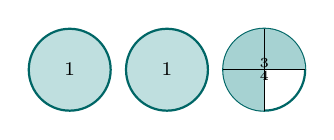
\begin{tikzpicture}[scale=0.65]
      \draw[fill=teal!25, draw=teal!80!black, thick] (0,0) circle (0.8cm);
      \node at (0,0) {\scriptsize $1$};
      \draw[fill=teal!25, draw=teal!80!black, thick] (1.9,0) circle (0.8cm);
      \node at (1.9,0) {\scriptsize $1$};
      \begin{scope}[shift={(3.8,0)}]
        \draw[draw=teal!80!black, thick] (0,0) circle (0.8cm);
        \fill[teal!35] (0,0) -- (0.8,0) arc (0:270:0.8) -- cycle;
        \draw (0,-0.8) -- (0,0.8); \draw (-0.8,0) -- (0.8,0);
        \node at (0,0) {\tiny $\frac{3}{4}$};
      \end{scope}
    \end{tikzpicture}\\[2pt]
    {\tiny\color{teal!95!black}\bfseries $2$ hình tròn nguyên và $\frac{3}{4}$ hình tròn}
  \end{tcolorbox}
\end{minipage}

\vspace{3mm}

% --- KHỐI 2: CHUYỂN ĐỔI QUA LẠI ---
\noindent
\begin{minipage}[t]{0.50\textwidth}
  \begin{tcolorbox}[
    enhanced,
    title={\footnotesize\bfseries\color{white}\faExchange\ 2. Chuyển hỗn số thành phân số},
    colback=purple!2!white,
    colframe=purple!70!black,
    arc=2.5mm, boxrule=0.8pt, top=1.8mm, bottom=1.8mm, left=2.2mm, right=2.2mm
  ]
    \footnotesize
    \begin{tcolorbox}[colback=white, colframe=purple!70!black, boxrule=0.6pt, arc=1.5mm, halign=center, top=1mm, bottom=1mm]
      {\scriptsize\bfseries\color{purple!90!black}$a\dfrac{b}{c} = \dfrac{a \times c + b}{c}$}
    \end{tcolorbox}
    $\bullet$ Tử số mới $=$ Phần nguyên $\times$ Mẫu $+$ Tử số cũ.\\
    $\bullet$ Mẫu số mới $=$ Giữ nguyên mẫu số cũ.\\
    \textit{VD:} $3\dfrac{2}{5} = \dfrac{3 \times 5 + 2}{5} = \dfrac{17}{5}$.
  \end{tcolorbox}
\end{minipage}%
\hfill
\begin{minipage}[t]{0.48\textwidth}
  \begin{tcolorbox}[
    enhanced,
    title={\footnotesize\bfseries\color{white}\faExchange\ 3. Chuyển phân số thành hỗn số},
    colback=orange!2!white,
    colframe=orange!80!black,
    arc=2.5mm, boxrule=0.8pt, top=1.8mm, bottom=1.8mm, left=2mm, right=2mm
  ]
    \footnotesize
    Áp dụng cho phân số có \textbf{tử số $>$ mẫu số}:\\
    $\bullet$ Thực hiện phép chia: $\text{Tử} : \text{Mẫu} = q$ (dư $r$).\\
    $\triangleright$ Thương $q$ làm \textbf{phần nguyên}.\\
    $\triangleright$ Số dư $r$ làm \textbf{tử số}, giữ nguyên mẫu số.\\
    \textit{VD:} $\dfrac{17}{5} \rightarrow 17:5 = 3$ dư $2 \Rightarrow \dfrac{17}{5} = 3\dfrac{2}{5}$.
  \end{tcolorbox}
\end{minipage}

\vspace{3mm}

% --- KHỐI 3: SƠ ĐỒ TƯ DUY ---
\noindent
\begin{tcolorbox}[
  enhanced,
  title={\footnotesize\bfseries\color{white}\faSitemap\ Sơ đồ tư duy: Các phép tính với hỗn số},
  colback=yellow!2!white,
  colframe=teal!85!black,
  arc=3mm, boxrule=0.9pt, top=1.8mm, bottom=1.8mm, left=1.5mm, right=1.5mm,
  halign=center
]
  \begin{tikzpicture}[
    scale=0.92,
    every node/.style={transform shape},
    root/.style={rectangle, rounded corners=5pt, fill=teal!85!black, text=white, font=\bfseries\footnotesize, inner sep=5pt, align=center},
    b1/.style={rectangle, rounded corners=4pt, fill=blue!12, draw=blue!75!black, text=blue!90!black, font=\bfseries\scriptsize, inner sep=4.5pt, align=center},
    b2/.style={rectangle, rounded corners=4pt, fill=green!15, draw=green!65!black, text=green!80!black, font=\bfseries\scriptsize, inner sep=4.5pt, align=center}
  ]
    \node[root] (core) at (0, 0.75) {\faCalculator\ TÍNH TOÁN VỚI HỖN SỐ};
    \node[b1] (m1) at (-4.7, -0.45) {\textbf{Cách 1: Đổi ra phân số rồi tính}\\[2pt](An toàn nhất cho mọi phép tính)};
    \node[b2] (m2) at (4.7, -0.45) {\textbf{Cách 2: Tính riêng nguyên và phân số}\\[2pt](Nhanh với phép cộng: $a\frac{b}{c} + d\frac{e}{f}$)};

    \draw[teal!85!black, thick, -{Stealth[length=2mm]}] (core) -| (m1);
    \draw[teal!85!black, thick, -{Stealth[length=2mm]}] (core) -| (m2);
  \end{tikzpicture}
\end{tcolorbox}

\vspace{3mm}

% --- KHỐI 4: SO SÁNH HỖN SỐ & BẪY TRẮC NGHIỆM ---
\noindent
\begin{minipage}[t]{0.54\textwidth}
  \begin{tcolorbox}[
    enhanced,
    title={\footnotesize\bfseries\color{white}\faBalanceScale\ So sánh hai hỗn số},
    colback=green!3!white,
    colframe=green!60!black,
    arc=2.5mm, boxrule=0.8pt, top=1.8mm, bottom=1.8mm, left=2.2mm, right=2.2mm
  ]
    \footnotesize
    $\bullet$ Hỗn số nào có \textbf{phần nguyên lớn hơn} thì lớn hơn.\\
    \textit{VD:} $4\dfrac{1}{5} > 3\dfrac{4}{5}$ (vì $4 > 3$).\\
    $\bullet$ Nếu \textbf{phần nguyên bằng nhau}: So sánh phần phân số.\\
    \textit{VD:} $2\dfrac{3}{5} > 2\dfrac{2}{5}$ (vì $\dfrac{3}{5} > \dfrac{2}{5}$).
  \end{tcolorbox}
\end{minipage}%
\hfill
\begin{minipage}[t]{0.44\textwidth}
  \begin{tcolorbox}[
    enhanced,
    title={\footnotesize\bfseries\color{white}\faExclamationTriangle\ Mẹo tránh bẫy trắc nghiệm},
    colback=red!2!white,
    colframe=red!70!black,
    arc=2.5mm, boxrule=0.8pt, top=1.8mm, bottom=1.8mm, left=2.2mm, right=2.2mm
  ]
    \footnotesize
    $\bullet$ Bẫy viết sai: $2\dfrac{5}{3}$ là \textbf{sai} vì phần phân số phải $< 1$. Phải chuyển thành $3\dfrac{2}{3}$.\\
    $\bullet$ Với phép nhân và chia hỗn số: \textbf{Bắt buộc} phải đổi ra phân số trước khi nhân/chia, tuyệt đối không nhân riêng phần nguyên!
  \end{tcolorbox}
\end{minipage}

\end{document}
